%\section{Performance of the FLAME Framework}
\label{sec:performance-flame}
FLAME is a agent-based modelling framework which generates an applications program. It manages the communications between agents through the Message Board Library and provide mechanisms in the model definition file (XMML) and the through the FAME API for the application developer to definite and optimise his application.

By design FLAME will generate both serial and parallel versions of an application. They both use the functions of the \textit{libmboard} to manage messages. It is \textit{libmboard} that performs the mapping of the application onto a parallel system. The parallel implementation of FLAME seeks to use an SPMD paradigm - each node of the parallel system is running essentially the same $program$. 

However given the nature of agent-based modelling and the FLAME implementation each nodal program could perform a very different sequence of instructions and function activations as it traverses its part of the state space. 

The two fundamental design features of FLAME are that all communications between agents takes place through a specified message board - a message repository - and that these message boards are distributed over the processing nodes of the parallel system. These message boards can be considered the data load and the agents themselves the computational load. In FLAME both these are distributed over the computational nodes.

However, although there may be some imbalance in computational load, with a reasonable initial data - agents - distribution, any imbalance should be small. The crucial element in the parallel implementation of FLAME is the distribution of the message boards over the system and their synchronisation.

It is clearly essential that the FLAME infrastructure does not impose a high overhead on the application. The \textit{Timer} package has been use to estimate the overhead of the FLAME infrastructure. The most important task performed by the FLAME framework is message and  message board management. Although applications make use of a variety of message board function - writing and reading messages from message boards - the message board synchronisation process is potentially the most costly.

Table \ref{table:overlap} gives details on the time taken by the FLAME framework to perform this synchronisation. Each row in the table gives the synchronisation time as a percentage of  the total elapsed time per iteration for the top five message boards in each group. The two left-hand columns of this show the basic synchronisation time. Even when combined it is clear the all the message board synchronisations are only taking 5\% of the total run time. Although we would expect to reduce this through some more detailed optimisation of the synchronisation algorithms and code, 5\% is considered to be an acceptable overhead.

\begin{table}[ht]
\centering
\begin{tabular}{|l|l|l|l|l|}\hline
              & \multicolumn{2}{c|}{No overlap} & \multicolumn{2}{c|}{Overlap} \\ \hline
Message board & Node 0 & Node 1 & Node 0 & Node 1 \\ \hline \hline
order & 3.3 & 2.9 & 3.0 & 2.2 \\ \hline
loan$\_$conditions & 0.1 & 0.2 & - & - \\ \hline
info$\_$firm & $<0.1$ & $<0.1$ & - & -  \\ \hline
order$\_$status & $<0.1$ & $<0.1$ & $<0.1$ & $<0.1$ \\ \hline
bank$\_$account$\_$update & $<0.1$ & - & $<0.1$ & $<0.1$ \\ \hline
eurostat$\_$send$\_$macrodata & - & 1.2 & - & -  \\ \hline
vacancies2 & - & - & $<0.1$ & -  \\ \hline
capital$\_$good$\_$request & - & - & $<0.1$ & $<0.1$ \\ \hline
capital$\_$good$\_$delivery & - & - & - & $<0.1$ \\ \hline 
\end{tabular}
\caption{Percentage of total time spent synchronising top nine message boards}
\label{table:overlap}
\end{table}

In the design of FLAME care has been taken to overlap communication and computation so that, as far as possible, agent functions are not waiting for data during their activation. This has been achieved by FLAME analysing the sending and receiving of messages defined in the model XMML file to push the start of communication (call to \texttt{MB$\_$SyncStart()}) as high as possible in the call tree (i.e.\ just after all messages of a particular type have been sent to the message board) and the wait for communication to complete (call to \texttt{MB$\_$SyncComplete()}) as low as possible (just before the messages are required).

To illustrate the effect of overlapping communication and computation a special version of FLAME that placed the calls to  \texttt{MB$\_$SyncStart} and \texttt{MB$\_$SyncComplete} as successive operations was run alongside the usual version. The timer package was used to time the \texttt{MB$\_$SyncComplete} functions in both cases and the results are given for the 5 longest elapsed times in Figure \ref{fig:overlap}. Runs were for a 16 region problem on 2 nodes for 40 iterations. 

\begin{figure}[ht]
 \centering
  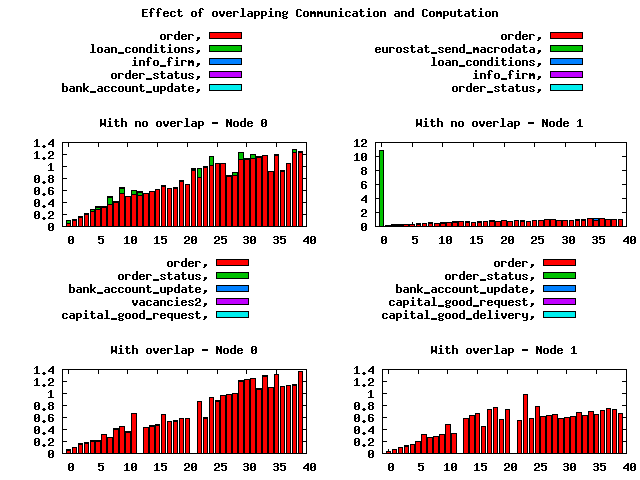
\includegraphics[width=450pt]{overlap.png}
 \caption{Elapsed times (s) for message board synchronisations with an without communication/computation overlapping}
 \label{fig:overlap}
\end{figure}

It is clear that the \texttt{eurostat$\_$send$\_$macrodata} message board is a significant beneficiary of overlapping. Looking at the state graph for the model shows that the messages are sent by the Eurostat agent very early in an iteration and read by the Government agents very late in the iteration.

The \texttt{order} message board benefits less since order messages are required very soon after they are sent (again from the state graph).






 
